\chapter{Versuchsaufbau}
In ein gemeinsames Schaltbild wird ein Instrumentenverstärker mit drei Operationsverstärkern aufgebaut und ein Instrumentenverstärker mit dem integrierten Instrumentenverstärker AD8226. Diese werden mit der Spannung $\pm 12\,\text{V}$ verbunden.

 \begin{figure}[h!]
                \centering
                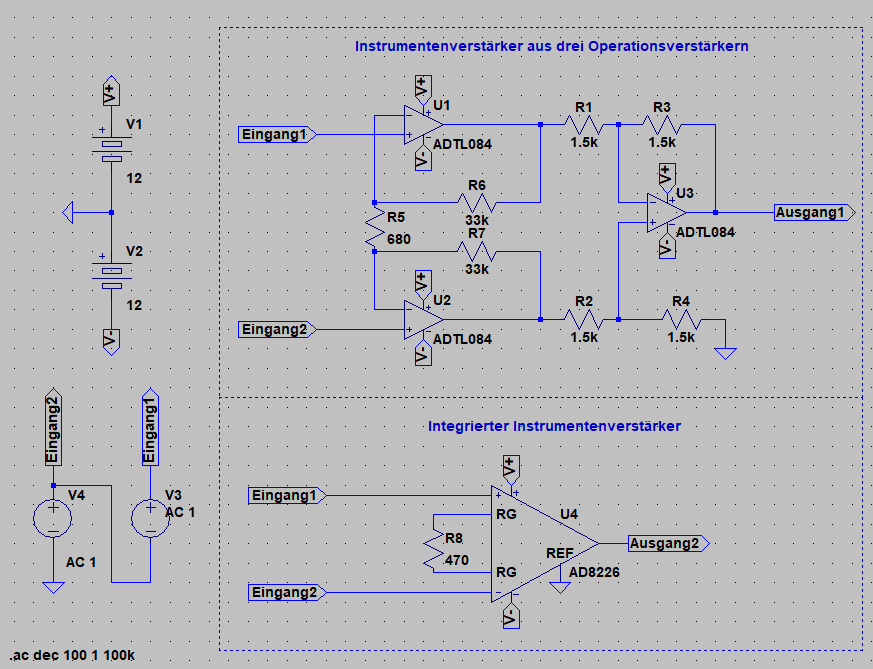
\includegraphics[width=1\linewidth]{schaltung.PNG}
                \caption{Aufbau der Schaltung der Instrumentenverstärker}
                \label{fig:schaltung}
            \end{figure}
            
Die in der Vorbereitung errechneten Werte sind in die Schaltung Abb. 2.1 integriert.
$$\,\text{R}_{8}=470\Omega$$
$$\,\text{R}_{6}=\,\text{R}_{7}=33\,\text{k}\Omega$$
$$\,\text{R}_{5}=680\Omega$$
Dieser erste Teil mit den Widerständen $\,\text{R}_5$ bis $\,\text{R}_7$ und den Operationsverstärkern $\,\text{U}_1$ und $\,\text{U}_2$ bildet den Differenzverstärker. Die Widerstände $\,\text{R}_1$ bis $\,\text{R}_4$ mit dem Operationsverstärker $\,\text{U}_3$ bilden den Subtrahierer der Schaltung. Die Widerstände $\,\text{R}_1$ bis $\,\text{R}_4$ wird der Wert 1,5 k$\Omega$ gegeben.
